\documentclass[runningheads,a4paper]{llncs} \usepackage[utf8]{inputenc}
\usepackage[hyphens]{url}
\usepackage{graphicx}
\usepackage{hyperref}
\usepackage{float}
\usepackage{eurosym}
\usepackage[normalem]{ulem}
\usepackage{alltt}
\usepackage{amssymb}
\usepackage{listings}
\usepackage{subfigure}
\setcounter{tocdepth}{3}

\usepackage{url}
\newcommand{\keywords}[1]{\par\addvspace\baselineskip
\noindent\keywordname\enspace\ignorespaces#1}

\begin{document}

\mainmatter  % start of an individual contribution

% first the title is needed
\title{Context-aware Querying for\\ Multimodal Search Engines}

% a short form should be given in case it is too long for the running head
\titlerunning{Context-aware Querying for Multimodal Search Engines}

\author{Jonas Etzold\inst{1} \and Arnaud Brousseau\inst{2} \and Paul Grimm\inst{1} \and Thomas Steiner\inst{2}}

\authorrunning{Context-aware Querying for Multimodal Search Engines}
% (feature abused for this document to repeat the title also on left hand pages)

% the affiliations are given next; don't give your e-mail address unless you
% accept that it will be published
\institute{Erfurt University of Applied Sciences, Germany, \email{\{jonas.etzold|grimm\}@fh-erfurt.de}
\and Google Germany GmbH, ABC-Str. 19, 20354 Hamburg, Germany,
\email{\{arnaudb|tomac\}@google.com}}

\maketitle

\begin{abstract}
Multimodal interaction provides the user with multiple modes of interacting with
a system, such as gestures, speech, text, video, audio, etc. A multimodal system allows for several distinct means for input and output of data. In this paper, we present our work in the context of the \mbox{I-SEARCH} project, which aims at enabling context-aware querying of a multimodal search framework including real-world data such as user location or temperature. We introduce the concepts of \emph{MuSeBag}, \emph{UIIFace}, and \emph{CoFind} as the core components behind the \mbox{I-SEARCH} multimodal user interface, which we evaluate via a user study. 

\keywords{Multimodality, Context Awareness, User Interfaces}
\end{abstract}

\section{Introduction}
The \mbox{I-SEARCH} project aims to provide a unified framework for multimodal content indexing, sharing, search and retrieval. This framework will be able to handle specific types of multimedia and multimodal content, namely text, 2D images, hand-drawn sketches, videos, 3D objects and audio files), but also real world information that can be used as part of queries. Query results can include any available relevant content of any of the aforementioned types. This is achieved through Rich Unified Content Annotation (RUCoD), a concept that we have introduced in~\cite{ijmis}. It becomes clear that a framework like \mbox{I-SEARCH} faces specific challenges with regards to the user interface (UI). Not only does it have to allow for the combination of multimodal queries, but it also has to do so on different devices, both desktop and mobile. This research being conducted in the context of a European research project, we have time constraints to take into account, hence, we cannot afford to develop two separate UI stacks for desktop and mobile. Instead, we show how using newly added features in the markup language HTML  we can kill these two flies with one stone.

The remainder of this paper is structured as follows: Section~2 presents related work, Section~3 introduces our chosen methodology, Section~4 goes into implementation details and presents some preliminary results, Section~5 presents the evaluation of a user study that we have conducted, Section~6 ends the paper with an outlook on future work and provides a conclusion.

\section{Related Work} \label{sec:related}
Many have been involved in research to improve user interfaces (UI) for search tasks in the last few years. They widely found evidence for the importance and special demand on the design of search UIs in order to achieve an effective and usable search~\cite{hearst2009},~\cite{quesenbery2008},~\cite{huangTsaiChang2009}). Especially with the emerge of the so-called Web 2.0 and the vast amount of user generated content, the raise of the big search engines like Google and Bing continued, and search became one of the main tasks in our daily Internet usage~\cite{quesenbergWeb2008}. This trend further increases the importance of the interaction with, and the design of search engines, and also raises the need for extending search tasks beyond textual queries on desktop systems. In this manner, Hearst~\cite{hearst2011} describes emerging trends for search interface design, which include that interfaces have to be more device-independent (i.e. also support mobile devices), and be able to support the creation of multimodal search queries where text can be enriched with multimedia and real-world data in order to deliver more precise results. With the development of multimodal search interfaces, also concepts for multimodal interaction, as defined by Nigay et al.~\cite{nigay}, become an important aspect to distribute all features of this new type of search interfaces to the user. Rigas~\cite{rigas2007} also found evidence that the use of multimodal features of a search interface, e.g. speech or graphs can support the usability of the whole search engine. In order to combine the efforts towards multimodal interaction, the World Wide Web Consortium (W3C) follows an approach to create a framework that is described by the W3C Multimodal Interaction Working Group with its work-in-progress specification of the ``Multimodal Architecture and Interfaces''~\cite{w3cMMI}. Therein, the framework is used to describe the internal structure of a certain interaction component, including the in- and outputs of the various interaction types based on XML. Serrano et al. further created the open interface framework~\cite{openinterface}, which allows for the flexible creation of combined interaction pipelines using several input channels (e.g. speech and touch). Other approaches to provide frameworks for multimodal interaction and interfaces are described by Sreekanth~\cite{sreekanth}, who uses a \textit{Monitor Agent} to collect events from different modalities and Roscher~\cite{roscher}, who uses the Multi-Access Service Platform (MASP), which implements different user interface models for each input modality and is able to combine them to more complex multimodal user interfaces including the synchronization of all inputs along the user interface models.

The possibility to generate more complex, but also more effective search queries with multimodal search interfaces, as well as the nature of the Internet as an environment where people can assist each other, make the integration of
collaborative interaction approaches for search engines interesting. Mainly the work of Morris~\cite{morris2007} and Pickens~\cite{pickens2008} described interesting ways of collaborative search approaches. They make use of a search
session and state variables in user profiles to transfers changes made in the interface of one user to all other collaborating users and vice versa. Further, the survey about collaborative Web search practices done by Morris~\cite{morris2008} as well as the status quo practices presented by Amershi~\cite{amershi2009} proof the need and practicability of collaborative search methods.

\section{Methodology}
In this Section, we present our methodology for context-aware querying of multimodal search engines, split up in three sub-tasks \emph{MuSeBag}, \emph{UIIFace}, and \emph{CoFind}.

\subsection{Multimodal Query Interfaces -- MuSeBag}
In order to create a visual platform for multimodal querying between user and search engine, the concept of \emph{MuSeBag} was developed. MuSeBag stands for \textbf{Mu}ltimodal \textbf{Se}arch \textbf{Bag} and designates the \mbox{I-SEARCH} UI. It comes with specific requirements linked with the need for users to use multiple types of input: audio files or stream, video files, 3D objects, hand drawings, real-world information such as geolocation or time, image files, and of course, plain text. This part of the paper shows the approach chosen to create MuSeBag.

Multimodal search engines are still very experimental at the time of writing. When building MuSeBag, we tried to look for a common pattern in search-related actions. Indeed, MuSeBag remains a search interface at its core. In order for users to interact efficiently with \mbox{I-SEARCH}, we needed a well-known interface paradigm. Across the Web, one pattern is used for almost any and all search related actions: the text field, where a user can focus, enter her query, and trigger subsequent search actions. From big Web search engines such as Google, Yahoo!, or Bing, to intranet search engines, the pattern stays the same. However, \mbox{I-SEARCH} cannot directly benefit from this broadly accepted pattern, as a multimodal search engine must accept a large number of query types at the same time: audio, video, 3D objects, sketches, etc. Some search engines, even if they do not have the need for true multimodal querying, still do have the need to accept input that is not plain text.

As a first example, we consider TinEye\footnote{\url{http://www.tineye.com/}}. TinEye is a Web-based search engine that allows for query by image content (QBIC) in order to retrieve similar or related images. The interface is split in two distinct parts: one part is a text box to provide a link to a Web-hosted image, while the second part allows for direct file upload (Figure~\ref{fig:tineye-ui}). This interface is a good solution for a search engine like TinEye (image input, image output), however, the requirements for \mbox{I-SEARCH} are more complex.

\begin{figure}[h!]
  \centering
    
\includegraphics[width=0.7\linewidth]{resources/tineye-UI.png}
  \caption{Screenshot of the TinEye user interface.}
  \label{fig:tineye-ui}
\end{figure}

As a second example, we examine MMRetrieval\footnote{\url{http://www.mmretrieval.net}}~\cite{mmretrieval}. It brings image and text search together to compose a multimodal query. MMRetrieval is a good showcase for the problem of designing a UI with many user-configurable options. For a user from outside the Information Retrieval field, the UI seems not necessarily clear in all detail, especially when field-specific terms are used (Figure~\ref{fig:mmretrieval-ui}).

\begin{figure}[h!]
  \centering
    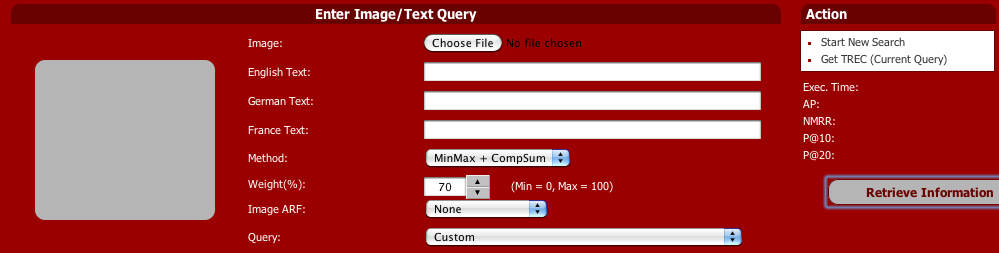
\includegraphics[width=0.7\linewidth]{resources/mmretrieval-UI.png}
  \caption{Screenshot of the MMRetrieval user interface.}
  \label{fig:mmretrieval-ui}
\end{figure}

Finally, we have a look at Google \textit{Search by image}\footnote{\url{http://googleblog.blogspot.com/2011/06/knocking-down-barriers-to-knowledge.html}}, a feature introduced in 2011 with the same UI requirements as MMRetrieval: combining text and image input. With the \textit{Search by image} interface, Google keeps the text box pattern (Figure~\ref{fig:search-by-image-box}), while preventing any extra visual noise. The interface is \emph{progressively disclosed} to users via a contextual menu when the camera icon is clicked.

\begin{figure}[h!]
  \centering
    
\includegraphics[width=0.7\linewidth]{resources/search-by-image-UI-box.png}
  \caption{Input for the \textit{Search by image} user interface.}
  \label{fig:search-by-image-box}
\end{figure}

Even if the \textit{Search by image} solution seems evident, it is still not suitable for \mbox{I-SEARCH} since the interface would require a high number of small icons: camera, 3D, geolocation, audio, video, etc.  As a result, we decided to adapt a solution that can be seen in Figure~\ref{fig:isearch-ui}. This interface keeps the idea of a single text box. It is enriched with text auto-completion as well as ``tokenization". By the term ``tokenization" we refer to the process of representing an item (picture, sound, etc.) with a token in the text field, as if it was part of the text query. We also keep the idea of \emph{progressive disclosure} for the different actions required by the various modes, e.g. uploading a picture or sketching something. The different icons are grouped together in a separated menu, close to the main search field.

\begin{figure}[h!]
  \centering
    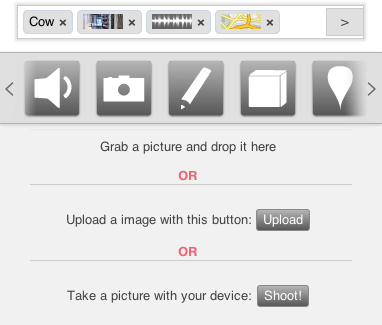
\includegraphics[width=0.4\linewidth]{resources/isearch-UI-mobile.png}
  \caption{First version of \mbox{I-SEARCH} interface.}
  \label{fig:isearch-ui}
\end{figure}

\subsection{Multimodal interaction -- UIIFace}
Interaction is an important factor when it comes to context-awareness and multimodality. In order to deliver a Graphical User Interface (GUI) that is able to facilitate all the possibilities of a multimodal search engine, a very flexible approach with a rich interaction methodology is needed. Not only the way search queries are build should be multimodal, also the interaction to generate and navigate in such a multimodal interface should be multimodal. Further, multimodal querying can also involve the way a user interacts with the system as part of the query. To target all those needs, we introduce the concept of \emph{UIIFace} (\textbf{U}nified \textbf{I}nteraction \textbf{I}nter\textbf{face}) as general interaction layer for context-aware multimodal querying. UIIFace describes a common interface between these interaction modalities and the graphical user interface (GUI) of \mbox{I-SEARCH} by providing a general set of interaction commands for the interface. Each input modality provides the implementation for parts of the commands or all commands defined by UIIFace. 

The idea of UIIFace is based on the open interface framework~\cite{openinterface}, which describes a framework for the development of multimodal input interface prototypes. It uses components that can represent different input modalities as well as user interfaces and other required software pieces in order to create and control a certain application. In contrast to this approach, UIIFace is a Web-based approach implemented on top of modern HTML5~\cite{html5} functionalities. Furthermore, it provides a command line interface to the Web-based GUI, which allows for the creation of stand-alone applications outside of the browser window. For the set of uni- and multimodal commands that can be used for \mbox{I-SEARCH} interfaces, the results of Chang~\cite{chang} as well as the needs derived from the creation of multimodal search queries are used.

\begin{figure}[h!]
  \centering
    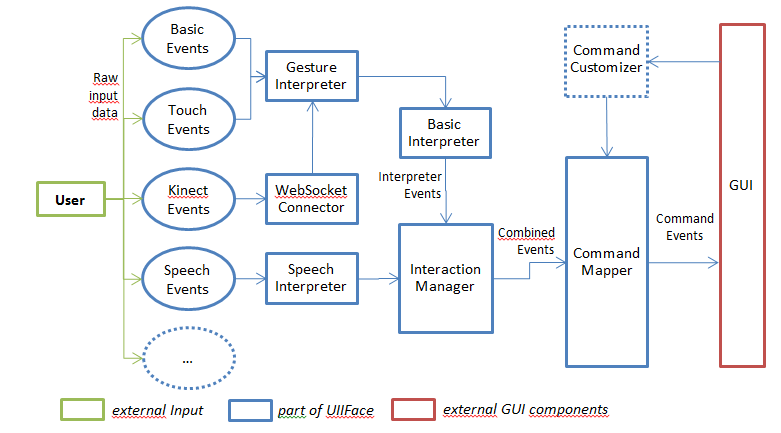
\includegraphics[width=0.8\linewidth]{resources/uiiface-structure.png}
  \caption{Schematic view on the internal structure of UIIFace.}
  \label{fig:uiiface}
\end{figure}

Figure~\ref{fig:uiiface} depicts the internal structure of UIIFace and shows the flow of events. Events are fired by the user's raw input. Gesture Interpreter determines defined gestures (e.g. zoom, rotate) found in the raw input. If no
gestures were found, the Basic Interpreter routes Touch and Kinect\footnote{A motion sensing input device by Microsoft for the Xbox 360 video game console.} events to basic cursor and keyboard events. Gestures, speech commands and basic mouse and keyboard events are then synchronized in the Interaction Manager and forwarded as Combined Events to the Command Mapper which maps the incoming events to the defined list of interaction commands that can be registered by any Web-based GUI. The Command Customizer can be used to rewrite the trigger event for commands to user specific gestures or other input sequences (e.g. keyboard shortcuts). This is an additional feature that is not crucial for the functionality of UIIFace, but that can be implemented at a later stage in order to add more explicit personalization features.

\subsection{Collaborative Search -- CoFind}
Another part of our methodology targets the increased complexity of search tasks and the necessity to collaborate on those tasks in order to formulate adequate search queries, which lead faster to appropriate result. The increased
complexity is primarily caused by the vast amount of unstructured data on the Internet and secondly by situations where the expected results are very fuzzy or hard to describe in textual terms. Therefore the CoFind (\textbf{Co}llaborative \textbf{Find}ing) approach is introduced as a collaborative search system, which enables real-time collaborative search query creation on a pure HTML interface. Real-time collaboration is well-known in the field of document editing (e.g. EtherPad\footnote{\url{https://github.com/ether/pad}}, Google  Docs\footnote{\url{https://docs.google.com/}}); CoFind applies the idea of collaborative document editing to collaborative search query composition.

CoFind is based on the concept of shared search sessions in which HTML content of the participants' local clients is transmitted within this session. In order to realize collaborative querying, the concept provides functions for activating collaborative search sessions, joining other online users' search sessions and managing messaging between participants of the search session. Figure~\ref{fig:cofind} shows how the parts listed in the following interact during the search process in order to create a collaborative search session:
\begin{description}
  \item [Session Manager] Controls opening / closing of collaborative search sessions.
  \item [Content Manager] Broadcast of user interfaces changes to all participants.
  \item [Messaging Manager] Broadcast of status / user messages to all participants.
\end{description}

\begin{figure}[h!]
  \centering
    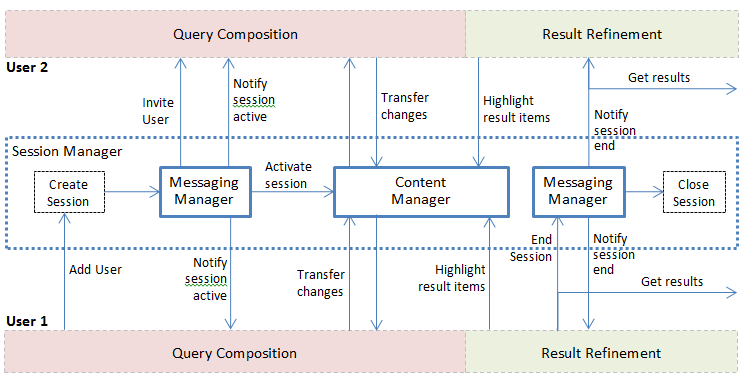
\includegraphics[width=0.75\linewidth]{resources/cofind-workflow.png}
  \caption{Schematic diagram of interaction between parts of CoFind.}
  \label{fig:cofind}
\end{figure}
 
The main flow of a collaborative search session can be described as follows: to join a collaborative search session initiated by a user A, a user B must supply the email address of user A. If user A is online and logged in, she receives an on-screen notification and needs to accept the collaboration request of the user B. Upon acceptance, a new session entry is created that stores all participants. Every time a change on the query input field or result set is occurs, the changed state is transferred to all participants. Each participant is able to search and navigate through the result set independently from the others, but selected results can be added to collaborative result set. The search session is closed after all users have left the session or have logged out from the system.

\section{Implementation Details}
The \mbox{I-SEARCH} GUI is built using the Web platform. HTML, CSS, and JavaScript are the three main building blocks for the interface. The rationale behind this choice is that \mbox{I-SEARCH} needs to be cross-browser and cross-device compatible, requirements fulfilled by CSS3~\cite{css3}, HTML5~\cite{html5} and the therein defined new JavaScript APIs that empower the browser in truly novel ways. However, our strategy also includes support for older browsers. When browsing the Web, a significant part of users do not have access to a cutting-edge Web browser. If a feature we use is not available for a certain browser version, two choices are available: either drop support for that feature if it is not important (e.g. drop visual shims like CSS shadows or border-radius), or provide alternate fallback solutions to mimic the experience. We would like to highlight that CSS and HTML are two standards that natively enable \emph{progressive enhancement} thanks to a simple rule: when a Web browser does not understand an HTML attribute, a CSS value or selector, it simply ignores it. This rule is the guarantee that we can build future-proof applications using CSS and HTML. Web browsers render the application according to their capabilities: older browsers render basic markup and styles, while modern browsers render the application in its full glory. Sometimes, however, we have to ensure that all users can access a particular feature. In this case, we use the principle of \emph{graceful degradation}, i.e. use fallback solutions when the technology stack does not support our needs in a certain browser.

\subsection{CSS3 Media Queries} 
The \mbox{I-SEARCH} project needs to be compatible with a large range of devices: desktop browsers, phones, and tablets. Rather than building several versions of \mbox{I-SEARCH}, we use CSS3 media queries\footnote{\url{http://www.w3.org/TR/css3-mediaqueries/}} to dynamically adapt the layout to different devices. 

\subsection{Canvas}
The \texttt{canvas} element in HTML5\footnote{\url{http://www.whatwg.org/specs/web-apps/current-work/multipage/the-canvas-element.html}} allows for dynamic, scriptable rendering of 2D shapes and bitmap images. In the case of \mbox{I-SEARCH}, we use \texttt{canvas} for user input when the query requires a user sketch, and also to display results in novel ways. The \texttt{canvas} element being a core element of \mbox{I-SEARCH}, it is crucial to offer a fallback solution for older browsers. We plan to do so by using FlashCanvas\footnote{\url{http://flashcanvas.net/}}, a JavaScript library, which adds the renders shapes and images via the Flash drawing API.

\subsection{HTML5 Audio and Video}
The \texttt{audio} and \texttt{video} elements make multimedia content a first class citizen in the Web browser, including scriptability, rotation, rescale, controls, CSS styles, and so forth. For \mbox{I-SEARCH}, this flexibility allows us to create interesting and interactive visualizations of search results. If \texttt{audio} and \texttt{video} are not available, we fall back to Flash\footnote{\url{http://www.adobe.com/products/flashplayer/}} to display media items to users.

\subsection{File API}
The file API ``provides an API for representing file objects in Web applications, as well as programmatically selecting them and accessing their data."\footnote{\url{http://www.w3.org/TR/FileAPI/}}. This is interesting in the case of \mbox{I-SEARCH}, since users are very likely to compose their query with local files, like audio files, pictures, etc. The file API allows for a new paradigm to deal with files, such as native support for dragging and dropping elements from the desktop to the \mbox{I-SEARCH} interface. This convenience feature is not crucial, an HTML file upload form serves as a fallback.

\subsection{Geolocation}
Context-aware search is one of the features of the \mbox{I-SEARCH} framework. This is particularly useful in the case of a user searching on a mobile device, as many mobile queries are location-based. HTML5 includes the geolocation JavaScript API that, instead of looking up IP address-based location tables, enables Web pages to retrieve a user's
location programmatically. In the background, the browser uses the device GPS if available, or computes an approximate location based on cell tower triangulation. The user has to agree for her location to be shared with the application.

\subsection{Sensors}
Another important aspect for context-awareness is the use of hardware sensors integrated or attached to different device types. These sensors are capable of retrieving the orientation and acceleration of a device or capturing the movements of a user in 3D space. With that knowledge the system is able to make assumptions about the user's
direct environment or to detect gestures, which further increases the overall context-awareness. Many of today's mobile devices have accelerometers and gyroscopes integrated that can be accessed through device-specific APIs. HTML5 supports events that target those sensors and defines unified events in the specification for the \emph{deviceorientation} (\textit{sic}) event~\cite{deviceOrientation}. Desktop sensors like the Kinect provide depth-information for tracking people in 3D space. These sensors do not yet have a common standard for capturing their data in a browser environment. For those sensors we have created a lightweight WebSocket-based~\cite{websockets} abstraction library.

\subsection{Device API}
With the Device API~\cite{deviceAPI} the W3C currently creates the next standard related to HTML5. It is mainly targeted to give Web browsers access to attached hardware devices of the client computer. Therefore the Media Capture API, which is a part of the Device API, will enable access to the microphone and the Web camera of the user. We use this API in combination with appropriate fallback routines in order to create audio queries as well as image queries captured on-the-fly.

\section{Evaluation}
To validate our interface design choices with real multimodal search tasks, we have conducted a user study. We went for a comparative study design to explore how usage of different media types would look like and how they would influence the success rate of search queries. As this user study was mainly focused on the user interface and user interaction parts of \mbox{I-SEARCH}, we assumed that the system always had a correct answer to the (limited) set of permitted queries, even if the real search back-end was not yet in operation at the time of writing. We therefore set the following hypotheses:
\begin{description}
  \item [(H1)] Most users will start a search query with just one media type.
  \item [(H2)] Search refinements will be done by adding / removing other media type.
  \item [(H3)] All media types are handled similarly.
\end{description}

For the user study we recruited seven participants (six male and one female) aged between 20 and 35. All participants were familiar with textual Web-based search. We asked all study participants to find three different items (sound of
a tiger, 3D model of a flower, image of a car). The participants were shown these items beforehand in their original format and were then instructed to query the system in order to retrieve them via \mbox{I-SEARCH}. For the study a Windows laptop with a capacitive touch display was used. Each participant was interviewed after the completion of the study. Our goal was to validate our interface design as well as to measure the impact of the possibility of multimodal search. In general, we observed that the concept of multimodal search was new and unfamiliar to all participants. Actually, before the user study all participants considered Web search equal to text-based search, and only by using \mbox{I-SEARCH} they became aware of the possibility to use different media types and of multimodal interaction at all (see Table ABCD). Our hypothesis (H1) was statistically not supported. It depends highly on the behavior of each individual person whether one or more search items or media types are used. In combination with (H2), one obvious conclusion of the participant interviews was that adding search items as well as customizing them has to be as easy as possible. The participants did not hit obstacles in using one special query modality, however stated that if a query modality was
difficult to use, they would replace it by using different query modalities, even if this implied that the search query would become complicated and challenging. The same conclusion applies to hypothesis (H3). In order to allow for  multimodal search queries, the following recommendations can be derived from our user study: 
\begin{enumerate}
  \item No query modality should be privileged.
  \item The handling of all search modalities should be as consistent as possible.
  \item Search refinement should be possible in the result presentation.  
\end{enumerate}

\section{Conclusion and Future Work}
(Tom)

\section{Acknowledgment}
This work is partly funded by the EU FP7 \mbox{I-SEARCH} project under project reference 248296.

\bibliographystyle{abbrv}
\bibliography{mmm2012}
\end{document}
